\documentclass[12pt]{article}
\newcommand{\ts}{\textsuperscript}

\usepackage[margin=1in]{geometry}
\usepackage{caption}
\usepackage{cite}
\usepackage{subcaption,graphicx}
\usepackage{lineno, blindtext}
\usepackage{float}
\usepackage{color}
\usepackage{graphicx}
\usepackage[hidelinks]{hyperref}
\usepackage{enumitem}
\usepackage{multicol}
\usepackage{fancyhdr}
\usepackage{times}
\usepackage{mathtools}
\usepackage{pdfpages}
\setlength{\parindent}{0pt}
\newcommand{\forceindent}{\leavevmode{\parindent=1em\indent}}
%\usepackage{siunitx}
\usepackage{chronology}

\usepackage[cache=false]{minted}


\title{MSE 486 Directed Study\\Report \#1 - Research\\ \bigskip \textbf{2 Player Texas Hold'em Poker\\Reinforcement Learning Python Bot}}
\author{Ryan Fielding - 301284210\\rafieldi@sfu.ca\\778.886.8199\\\\Supervisor: Dr. Ahmad Rad, Ph.D.\\Associate Director, School of Mechatronic Systems Engineering,\\Simon Fraser University}
\date{May $30^{th}$, 2020}

\begin{document}

\maketitle
\newpage

{\Large \textbf{Abstract\\\\}}
This paper outlines the project progress for a directed study in machine learning, through implementation and development of an AI based bot ('RLPlayer') to learn and understand different strategies to play poker. Particularly, the game of Texas Hold'em will be the basis for this project, potentially beginning with Leduc Hold'em since it is a much simpler version of the game.\\\\
To initiate the project, the first couple weeks will be dedicated to project research, pertaining to coding language, type of machine learning to implement, project goals, requirements and more. Implementation and development will be done in Python, through the AI of reinforcement learning.\\\\
To elaborate on the overall development, first, a basic poker environment will be initialized. There is no need to develop this from scratch as there are plenty of sources to implement a gaming environment in many languages. Following, basic game playing bots will need to be setup, as well as strategic bots and honest bots. Each level of trained bot will get more and more advanced.\\\\
In parallel, to satisfy the learning outcomes of this course as well as provide a sound understanding of machine learning, research pertaining to neural networks, types and architectures of machine learning, and intensive research involving reinforcement learning will be completed. Primarily during the first few weeks of the semester. Following, an implementation period will ensue to initiate environment setup and inital machine learning implementation. Lastly, the two phases will tie together to merge research and implemenation through multiple stages of training, with various parameters and according to different strategies, resulting in a well developed reinforcement learning poker playing bot.\\\\
Training these bots will mostly consist of self play and reward based learning, however other strategies will be researched, including that of DeepStack, Libratus, Pluribus and many others that are successfully based on machine learning. The reason for two player poker, instead of 3, 4 or even 6, is because with a lower number of players at play, a rule based gaming strategy is far more effective, and much easier to implement and train. As the number of players increase, the game becomes a multi-player game that requires more sophisticated strategies and potentially even player modelling.\\\\
In terms of technical specifics, Python and PyTorch will be used since it is the most user friendly language, however the core of PyTorch is written in C++, so as to preserve high speeds. In terms of computationally intensive neural network training, rather than purchase of a high quality GPU, use of CUDA to run on a Mac OS GPU, or many other hardware solutions, Google Colab. will be used since it enables the use of free GPU's for training of python neural networks for up to 12 hours \cite{colab}.

\newpage
\tableofcontents
\listoffigures
\newpage

\section{Background}
The complex game of poker requires reasoning with hidden information. When one plays a game, not only do they quantify the value of their own hand, they also aim to predict what cards the opposing players hold. Other players can even bet high when they're hand is not valuable at all, a strong tactic called \textit{bluffing}. Additionally, there are other factors that weigh in, including pot size, call size, remaining stack and more. For background information on Texas Hold'em and how it is played, see the reference \cite{tex}.\\\\
\begin{figure}[H]
    \centering
    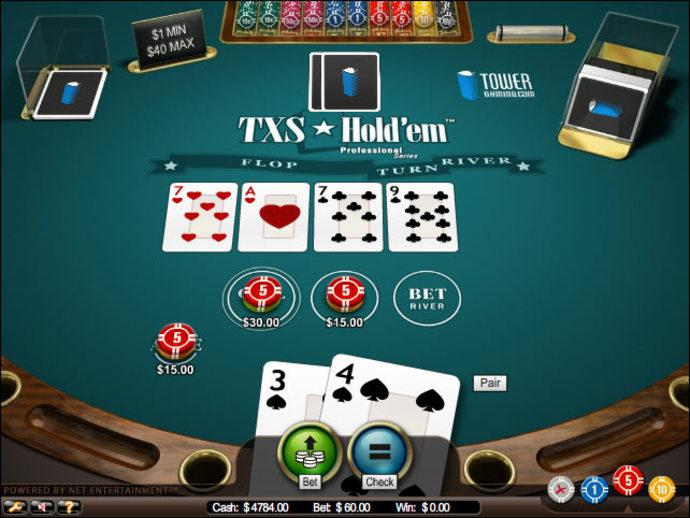
\includegraphics[width=.70\linewidth]{figures/texas.jpg}
    \caption{Online Texas Hold'em}
    \label{fig:tex}
\end{figure}
Two player Texas Hold'em presents an excellent opportunity to implement machine learning, as rule based strategies work fairly well, according to many experienced sources \cite{ai}. Game theory, with higher numbers of players, is far less helpful. Additionally, this becomes incredibly computationally expensive as it drastically increases the number of possibilities, making it much harder to make a sound decision at the time of it's turn. Bots known as Libratus and DeepMind's Go bot used 100 CPU's and 2000 CPU's, respectively \cite{ai}. However, a much less expensive AI has been developed, known as \textit{Pluribus}, which only required 2 CPU's to run. It was developed via reinforcement learning and self play, and such a tactic will most definitely be employed for the development of this project. 

\section{Research}
\subsection{Machine Learning and Neural Networks}
In order to achieve an in depth understanding of neural networks and machine learning, the course \textit{Intro to Deep Learning with PyTorch} on Udacity has been selected. Over the course of the first 4 weeks of this semester, the module \textit{Introduction to Neural Networks} has been completed, which outlines the concepts behind neural networks and how they are trained and tuned. This section will not dive into explaining the many concepts of neural networks, but will elaborate on how reinforcement learning applies to the game of poker and presumed topics that will need to be implemented.
\subsubsection{Udacity Course Concepts}
Luis Serrano, a course developer, guides the user through many of the common concepts of neural networks, including, but not limited to, the following:

\begin{itemize}
	\item Classification problems - linear boundaries and higher dimensions
	\item Perceptrons- non linear, perceptron algorithm,
	\item Error Functions - log-loss error function, discrete vs continuous
	\item Softmax, One-Hot Encoding
	\item Probabilities, Cross-Entropy
	\item Logistic regression, gradient descent
	\item Non-linear models, neural network architecture 
	\item Feedforward and backpropogation
	\item Training optimization, testing, over and under fitting
	\item Early stopping, regularization, dropout
	\item Local minima, random restart, vanishing gradient, momentum and many other common concepts
\end{itemize}
The course provides a good understanding of the concepts of neural networks, but does not dive deep into the concepts around reinforcement learning. It then goes to discuss the proper implementation of a neural network in PyTorch, but that will be explored throughout the implementation phase of this course (weeks 4-8).

\subsection{Reinforcement Learning}
\subsubsection{Why RL?}
The motivation for reinforcement learning (RL) lies in it's low computational expensiveness. Imagine you are playing chess, before you make a move, you are thinking what all the other player's potential moves are, even 2 or 3 moves ahead of the present. For a computer to do this, in a game with many possibilities and many players, it is incredibly expensive to do in a short period of time. Reinforcement learning is "an area of machine learning concerned with how software agents ought to take actions in an environment in order to maximize the notion of cumulative reward" \cite{rl}.
\begin{figure}[H]
    \centering
    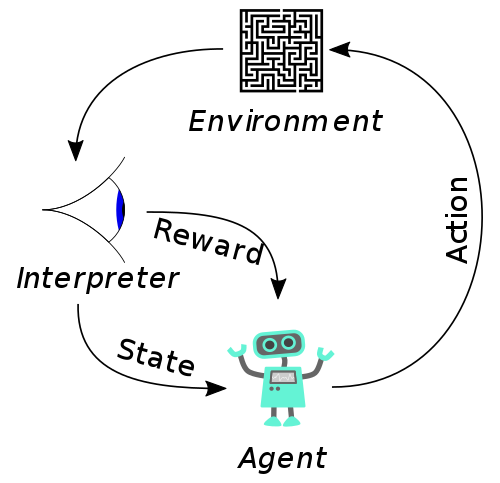
\includegraphics[width=.50\linewidth]{figures/rel.png}
    \caption{A Typical Reinforcement Learning Approach \cite{rl}}
    \label{fig:rl}
\end{figure}
If you are familiar with the game of poker, the image shown above is nearly directly applicable to the game. Thus, implementing this type of learning, coupled with iterative self play, can lead to a very powerful poker playing bot, especially in two player poker. Potential for implementation in more than two player poker may be explored and tested depending on effectiveness of that of two player.
\subsubsection{Elements of RL}
The reference listed in \cite{rlref} provided an incredibly well written introduction to reinforcement learning, hence most of the following information can be referenced there.
In addition to an agent, an environment, and the other aspects listed in the previous sections, the following list discusses the other main elements of RL.
\begin{itemize}
	\item \textit{A policy:} essentially defines the rules of the agent. For example, you cannot bet when it is not your turn, or if you've folded your cards. The agent's possible actions at any given state.
	\item \textit{A reward:} the goal of the agent. Basically, a reward is received by the agent from the environment upon every single discrete change in state. The agent's sole goal is to maximize the reward's it receives. Of course in the game of poker, this reward will be a high value if the agent wins a hand, and low if it loses, but not too low if it folds without losing any money, for example.
	\item \textit{A value function:} instead of an instant reward, the agent must also consider the effect of it's actions in the long run, quantified by the value function. For example, a state may have a low reward but have a high value, since it generally induces other states that have high rewards. In the case of poker, this is analogous to a player betting high when they have a very low stack. They may not have much money to bet, thus each bet has a low reward, but assuming they win the hand, the action of betting will have a high value as they will make money in the end. Value estimation is essentially the most important aspect to RL, as it determines how the agent will choose it's course of action.
	\item \textit{A model:} this element essentially mimics the environment to predict how it will change in response to an action, before actually taking that action. Since the game of poker is nearly impossible to model because it is a game of imperfect information, and it would be incredibly difficult to model different players during gameplay, this will not be included in the poker RL implementation.
\end{itemize}
\subsection{Deep Q Learning (Deep RL)}
Q learning aims to iteratively populate a 2D matrix of Q values based on current environment states and performing actions. It essentially uses trial and error to map an action to a state and output the reward, thus quantifying the value of certain actions given a state. This type of learning uses the Bellman equation to create a Q learning function \cite{q}. After finding the optimal Q matrix, the agent will pick it's action at any given state by finding the highest Q value for that state. This works well for low dimensional problems, but highly dimensional problems render this method impractical, hence the introduction of Deep Q Learning.\\\\
Deep Q Learning, on the other hand, uses a neural network to predict the reward at any given state. In the game of poker, there is no notion of how many states there will be - player A could bet X amount at any given moment, player C could fold, etc. This is another reason this method works effectively for high dimensional games. Lastly, instead of a 2D matrix to store all possible Q values, it uses a Q network that takes the current state as input and outputs Q values for all possible actions (bet, call, fold, bluff, raise). The figure below displays an excellent visual understanding.
\begin{figure}[H]
    \centering
    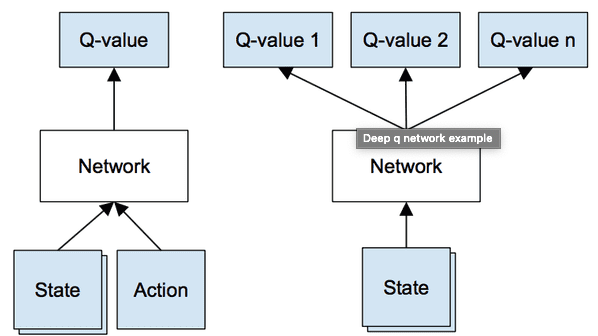
\includegraphics[width=.70\linewidth]{figures/q}
    \caption{Q Learning vs Deep Q Learning \cite{q}}
    \label{fig:q}
\end{figure}
Applying this to the game of poker will be tedious and trivial, however in \cite{q}, the algorithm performed very well at approximating a Nash Equilibrium for two player head's up push-or-fold poker - a very simplified version. It will most definitely be explored 
\subsubsection{Overall Architecture - DQN}
To provide a better visual understanding of what the integrated system with the deep Q network (DQN) will look like, see the figure below.
\begin{figure}[H]
    \centering
    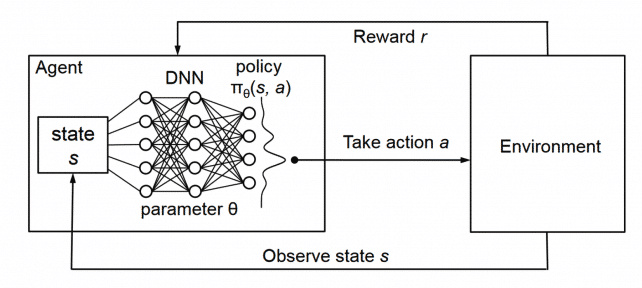
\includegraphics[width=.80\linewidth]{figures/qsys}
    \caption{DQN RL Architecture \cite{qsys}}
    \label{fig:q}
\end{figure}
For the RLPlayer, the agent, to make a decision on what action to take, the game state will be passed through the feedforward trained deep Q network upon every single change of state (after each player's turn and on the flop, turn, river - see \cite{gloss} for poker terminology). Of course, the DQN will be trained through self play, until an optimal poker bot AI converges. Appendix \ref{dqnmodel} displays the few lines of code written in Keras (another python ML library, similar to PyTorch) to build a basic 5 layer neural network.
\subsubsection{State Encoding}
One cannot simply pass the notions of state to the DQN as how they are represented to humans, all aspects of state must be encoded - or quantified as numbers. Instead of a player's hand of an 8 of Clubs and 10 of Clubs, this must be converted to a vector that can be passed into the DQN. The figure below from \cite{q} displays an example of \textbf{one-hot encoding} for this hand.
\begin{figure}[H]
    \centering
    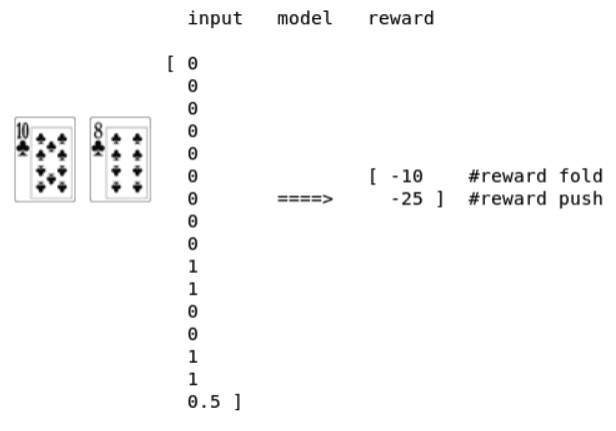
\includegraphics[width=.50\linewidth]{figures/enc}
    \caption{Example of Hand One-Hot Encoding \cite{q}}
    \label{fig:enc}
\end{figure}
This example contains rewards for the simplified game of heads up push-or-fold poker. There are many more states that are required to encode for 2+ player texas hold'em, such as:
\begin{itemize}
	\item RLPlayer hand
	\item Community cards
	\item Pot size
	\item RLPlayer stack size (amount of money)
	\item Opponents' stack size
	\item Number of opponents who have not folded
	\item Minimum bet to play
	\item Blind sizes
\end{itemize}
These are the majority of the states that will need to be encoded, however some are already in numerical form, such as the pot size, for example \$1,000, or players remaining, 3. Encoding is important as it represents how the DQN interprets and understands the game.
\subsubsection{Reward Signal - Bot Strategy}
The core \textbf{strategy} of the RLPlayer is based around the construction of the reward signal, or function. It determines what actions produce more rewards, affects the value function, Q values, and thus dictates how the player will play. It may lead to an aggressive strategy, a passive one, or others. The following equations represent a general expression of the function for Q.
\begin{equation}
	Q(s,a) = r + \gamma max_{a'} (s',a')
\end{equation}
Which implies that the Q value is equal to the immediate reward plus the future discounted ($\gamma$) reward for the most optimal action (\textit{a}), at a given state (\textit{s}). For backpropogation of our DQN, the Q learning function below can properly update Q values after performing an action. 
\begin{equation}
	Q_{t+1}(s_t , a_t) = Q_t(s_t,a_t) + \alpha ((r_{t+1}) + \gamma max_a Q_t(s_{t+1},a) - Q_t(s_t,a_t))
\end{equation}
Where $\alpha$ represents the learning rate. These equations, from \cite{q}, encompass the general concept of deep Q reinforcement learning through self play - performing actions, observing the changes in state and tuning the decision process based off the reward from these observations. Although they will not be used directly since DQN features a deep neural network to predict the Q value of an action, they are the base concept of Q learning. This is also know as a \textbf{Markov Decision Process}. Chapter 3 of \cite{rlref} greatly discuss this entire subject. Appendix \ref{dqnNN} displays just how simple it is to build a DQN in PyTorch.
\section{Implementation Progress}
Along with research, time has been put into the setup and testing of the chosen poker environment, to ensure feasibility of a properly functioning poker playing game. Once this is tested, time can be spent investigating PyTorch and it's integration to the poker bot and it's environment for training through self play.
\subsection{PyPokerEngine}
After exploring many options online, a well developed poker game engine written in Python has been chosen to utilize for the environment. The library can be found on GitHub \cite{pokergit} as well as supporting documentation for reinforcement learning users \cite{pokerdoc}, another reason it was chosen for this project. You can play against your AI via a console, through a GUI, or run a simulation of any number of rounds of AI vs AI, or a combination of bots. The library comes with built in bots, such as a fish player, fold player, random and honest players, which will be used for the training of our reinforcement learning (RL) bot. The following code displays just how simple it is to setup an RL bot \cite{pokergit}.
\begin{minted}[
frame=lines,
framesep=2mm,
baselinestretch=1.2,
fontsize=\footnotesize,
linenos
]{python}
from pypokerengine.players import BasePokerPlayer
from pypokerengine.api.emulator import Emulator
from pypokerengine.utils.game_state_utils import restore_game_state

from mymodule.poker_ai.player_model import SomePlayerModel

class RLPLayer(BasePokerPlayer):

    # Setup Emulator object by registering game information
    def receive_game_start_message(self, game_info):
        player_num = game_info["player_num"]
        max_round = game_info["rule"]["max_round"]
        small_blind_amount = game_info["rule"]["small_blind_amount"]
        ante_amount = game_info["rule"]["ante"]
        blind_structure = game_info["rule"]["blind_structure"]
        
        self.emulator = Emulator()
        self.emulator.set_game_rule(player_num, max_round, small_blind_amount, ante_amount)
        self.emulator.set_blind_structure(blind_structure)
        
        # Register algorithm of each player which used in the simulation.
        for player_info in game_info["seats"]["players"]:
            self.emulator.register_player(player_info["uuid"], SomePlayerModel())

    def declare_action(self, valid_actions, hole_card, round_state):
        game_state = restore_game_state(round_state)
        # decide action by using some simulation result
        # updated_state, events = self.emulator.apply_action(game_state, "fold")
        # updated_state, events = self.emulator.run_until_round_finish(game_state)
        # updated_state, events = self.emulator.run_until_game_finish(game_state)
        if self.is_good_simulation_result(updated_state):
            return # you would declare CALL or RAISE action
        else:
            return "fold", 0
\end{minted}
Where the \textit{declare\_actions} function is where the bot will make decisions on which actions to take based off the feedforward results of the trained neural network.

\subsection{PyPokerGUI}
Playing poker against a tuned AI bot through a console is a tedious and unrealistic task. After spending hours training an AI to play poker, one should be able to test it in an environment that resembles that of a real casino, hence the implementation of GUI (guided user interface) support for the \textit{PyPokerEngine}, called the \textit{PyPokerGUI} \cite{pokergui}. All settings exist in a \textbf{.yaml} file to configure and setup a localhost server to run the python module in any browser. Invoking the following command through a terminal can start the server and initiate the game engine GUI:\\\\
\textbf{python3 -m pypokergui serve poker\_conf.yaml --port 8000 --speed moderate}\\\\
The following figure displays a basic two player game of poker in a browser window:
\begin{figure}[H]
    \centering
    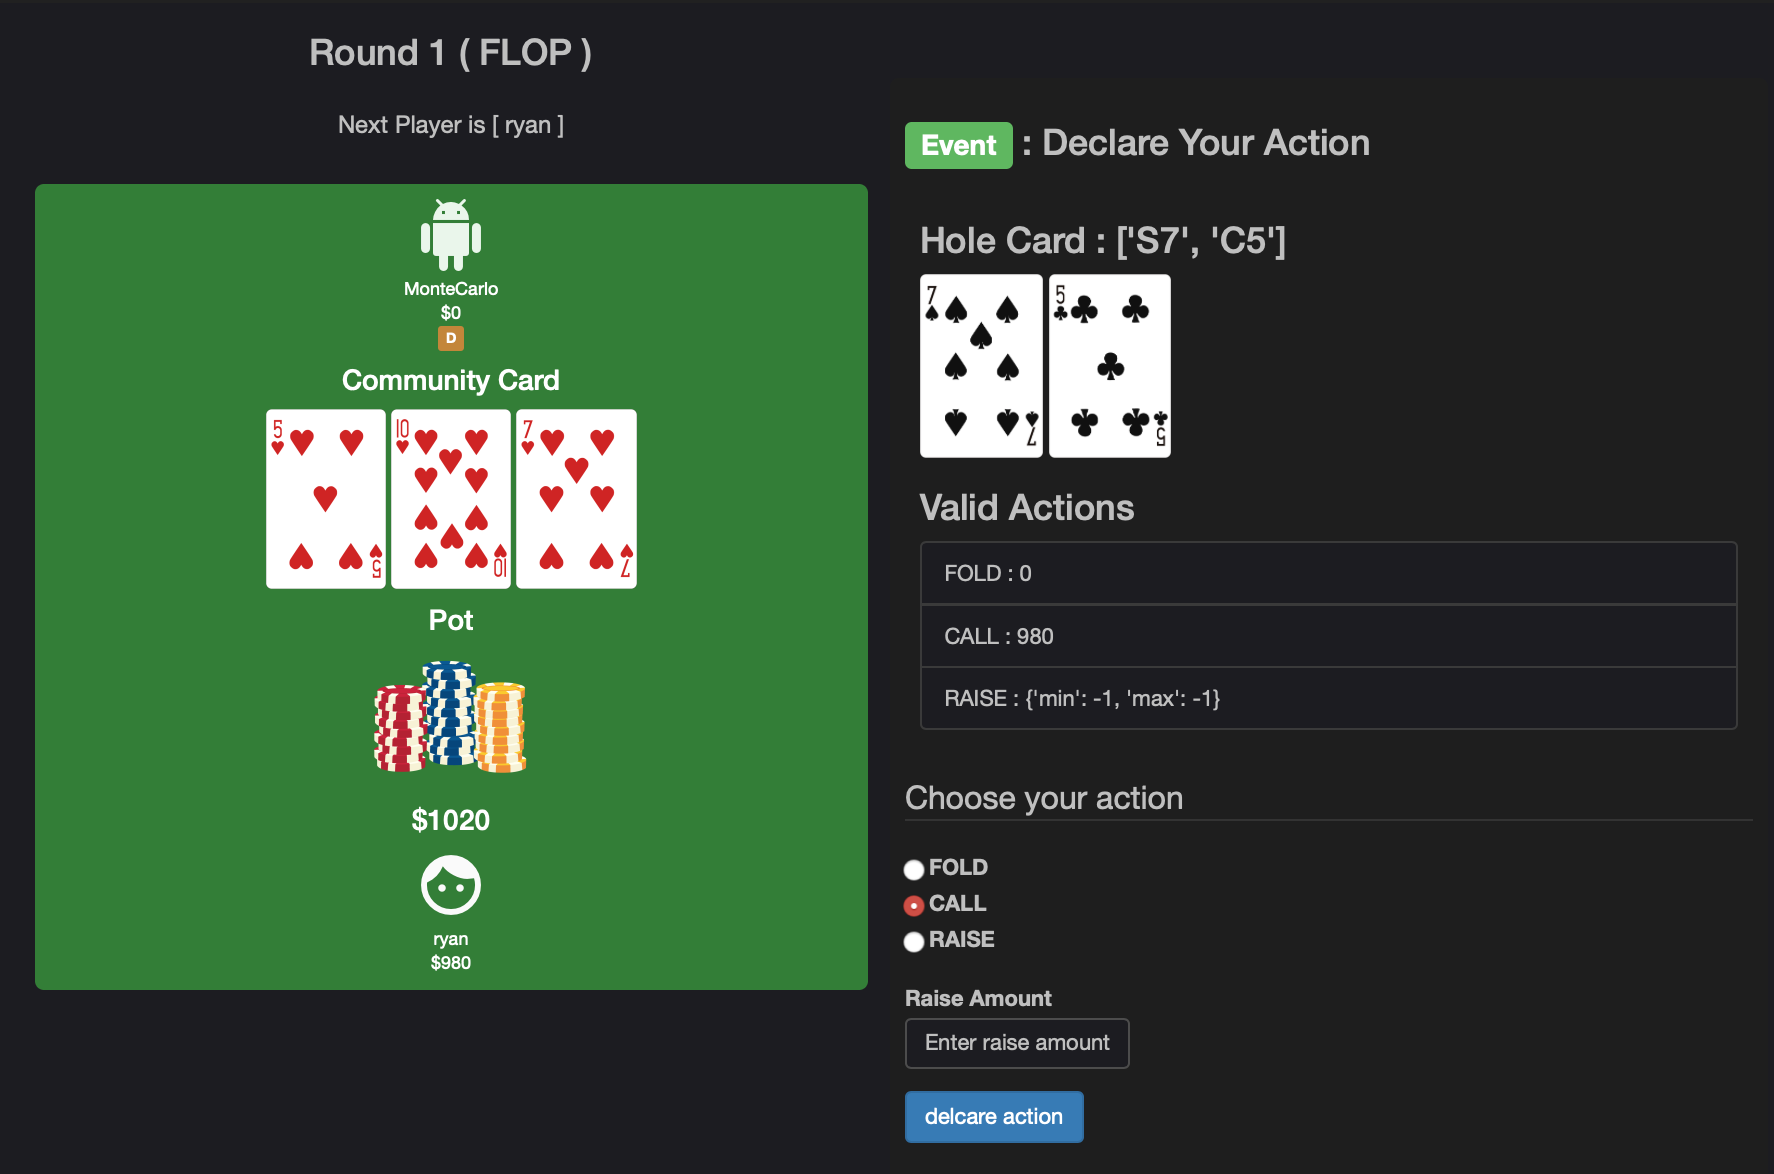
\includegraphics[width=.80\linewidth]{figures/gui}
    \caption{PyPokerGUI Example}
    \label{fig:gui}
\end{figure}
Of course, the game settings can be modified in the \textbf{.yaml} file to play multiple players of different types, different blind sizes, and more. This ultimately provides an excellent testing method for our trained neural network.
\subsection{Training Simulation}
In order to train the neural network, another method of testing or simulation must be readily available to run at high speeds that does not require user input. Hence, just a few following lines can be written in a Python script to begin a simulation of any number of games of poker, while consistently displaying the results.
\begin{minted}[
frame=lines,
framesep=2mm,
baselinestretch=1.2,
fontsize=\footnotesize,
linenos
]{python}
from pypokerengine.api.game import setup_config, start_poker
config = setup_config(max_round=10, initial_stack=100, small_blind_amount=5)
config.register_player(name="p1", algorithm=FishPlayer())
config.register_player(name="p2", algorithm=HonestPlayer())
config.register_player(name="p3", algorithm=RLPlayer())
game_result = start_poker(config, verbose=1)
\end{minted}
Some example results can be seen below:
\begin{minted}[
frame=lines,
framesep=2mm,
baselinestretch=1.2,
fontsize=\footnotesize,
linenos
]{python}
Started the round 10
Street "preflop" started. (community card = [])
"p1" declared "call:10"
"p2" declared "call:10"
"p3" declared "call:10"
Street "flop" started. (community card = ['H7', 'C7', 'C9'])
"p2" declared "call:0"
"p3" declared "call:0"
"p1" declared "call:0"
Street "turn" started. (community card = ['H7', 'C7', 'C9', 'H6'])
"p2" declared "call:0"
"p3" declared "call:0"
"p1" declared "call:0"
Street "river" started. (community card = ['H7', 'C7', 'C9', 'H6', 'HK'])
"p2" declared "call:0"
"p3" declared "call:0"
"p1" declared "call:0"
"['p2']" won the round 10 (stack = {'p1': 90, 'p2': 150, 'p3': 60})
\end{minted}
This simulation will be the core of training the RLPlayer - the neural network. Upon every single action (represented by each new line in the code above) , the player will backpropogate through it's network to tune the gains and minimize the error function, until a best fit is reached.
\subsection{PyTorch}
There are many libraries that implement the many various concepts and architectures of machine learning in Python, such as TensorFlow, Theano, PyTorch, and more. PyTorch has been chosen as it is the most user friendly, while it still preserves high speeds as it's core is written in C++. Development of the reinforcement learning poker player, implementation and training has not yet begun as it will take place during phase 2.
\subsection{Google Colab}
Google Colaboratory (Colab) allows anyone to deploy Python projects on remote servers with powerful GPU's. By merely inputting a link to a Github repository, one can execute computationally expensive programs even though they do not have direct access to hardware, through Colab. It begins with a free trial and then has a fee that is pay per use. This will be explored after a few tests of training the RLPlayer on a basic Mac OS CPU to better understand just how expensive training really is.

\section{Other Information}
\subsection{Timeline}
\begin{chronology}[3]{1}{15}{\textwidth}
\event{1}{Project Kick-off}
\event[1]{3}{Research}
\event[2]{4}{Environment Development}
\event{4}{Basic Environment and Bots Implemented}
\event{6}{Console Based UI Gameplay for Testing}
\event[4]{6}{RL Dev. and Training}
\event[5]{10}{Training and Testing}
\event{7}{Revision 1. Complete - RL}
\event{8}{More Advanced RL AI Bot}
\event[10]{14}{Testing, Training, Competitive Play}
\event{14}{Project Completion}
\event[14]{15}{Documentation}

\end{chronology}
\textbf{Project Timeline for the Summer 2020 Semester, by Week}\\

\subsection{Meeting Schedule}
Weekly meetings will be held at 11am PT, recurring weekly on Tuesdays.

% ADD BIBLIOGRAPHY
\newpage
\begin{flushleft}
\nocite{*}
\bibliographystyle{IEEE/IEEEtran}
\bibliography{IEEE/IEEEabrv,IEEE/biblio}
\end{flushleft}

%APPENDICES
\bigskip
\Large{\textbf{Appendices}}
\appendix
\section{Heads Up Push-or-Fold DQN Model}
\label{dqnmodel}
\normalsize
A basic 5 layer neural network written using Keras in Python.
\begin{minted}[
frame=lines,
framesep=2mm,
baselinestretch=1.2,
fontsize=\footnotesize,
linenos
]{python}
def preflop_model():

    input_n = Input(shape=(16,), name="input")

    x = Dense(32, activation='relu')(input_n)
    x = Dense(64, activation='relu')(x)
    x = Dense(16, activation='relu')(x)
    out = Dense(2)(x)
    model = Model(inputs=[input_n], outputs=out)
    model.compile(optimizer='adam', loss='mse')

    return model
\end{minted}

\section{Basic PyTorch NN}
\begin{minted}[
frame=lines,
framesep=2mm,
baselinestretch=1.2,
fontsize=\footnotesize,
linenos
]{python}
from torch import nn
class Network(nn.Module):
    def __init__(self):
        super().__init__()
        
        # Inputs to hidden layer linear transformation
        self.hidden = nn.Linear(784, 256)
        # Output layer, 10 units - one for each digit
        self.output = nn.Linear(256, 10)
        
        # Define sigmoid activation and softmax output 
        self.sigmoid = nn.Sigmoid()
        self.softmax = nn.Softmax(dim=1)
        
    def forward(self, x):
        # Pass the input tensor through each of our operations
        x = self.hidden(x)
        x = self.sigmoid(x)
        x = self.output(x)
        x = self.softmax(x)
        
        return x
\end{minted}

\section{Basic PyTorch DQN}
\label{dqnNN}
\begin{minted}[
frame=lines,
framesep=2mm,
baselinestretch=1.2,
fontsize=\footnotesize,
linenos
]{python}
class DQN(nn.Module):

    def __init__(self, h, w, outputs):
        super(DQN, self).__init__()
        self.conv1 = nn.Conv2d(3, 16, kernel_size=5, stride=2)
        self.bn1 = nn.BatchNorm2d(16)
        self.conv2 = nn.Conv2d(16, 32, kernel_size=5, stride=2)
        self.bn2 = nn.BatchNorm2d(32)
        self.conv3 = nn.Conv2d(32, 32, kernel_size=5, stride=2)
        self.bn3 = nn.BatchNorm2d(32)

        # Number of Linear input connections depends on output of conv2d layers
        # and therefore the input image size, so compute it.
        def conv2d_size_out(size, kernel_size = 5, stride = 2):
            return (size - (kernel_size - 1) - 1) // stride  + 1
        convw = conv2d_size_out(conv2d_size_out(conv2d_size_out(w)))
        convh = conv2d_size_out(conv2d_size_out(conv2d_size_out(h)))
        linear_input_size = convw * convh * 32
        self.head = nn.Linear(linear_input_size, outputs)

    # Called with either one element to determine next action, or a batch
    # during optimization. Returns tensor([[left0exp,right0exp]...]).
    def forward(self, x):
        x = F.relu(self.bn1(self.conv1(x)))
        x = F.relu(self.bn2(self.conv2(x)))
        x = F.relu(self.bn3(self.conv3(x)))
        return self.head(x.view(x.size(0), -1))
\end{minted}


\end{document}
